%!TEX root = planning.tex
\section{COCOMO: effort \& cost estimation}
\subsection{Overview} % (fold)
\label{sub:cocomo_overview}
The COCOMO II Cost Estimation Model is a complex estimation technique used 
by thousands of software engineers all over the world. \\
It's used to estimate the effort cost of a software engineering project.
The core of COCOMO II is the use of the Effort Equation to estimate the number
of Person/Month required to develop a complex project.

We have used this file as reference: \\ 
\url{http://csse.usc.edu/csse/research/COCOMOII/cocomo2000.0/CII_modelman2000.0.pdf}

\subsection{Scale Drivers} % (fold)
\label{sub:scale_drivers}
\begin{figure}[h]
    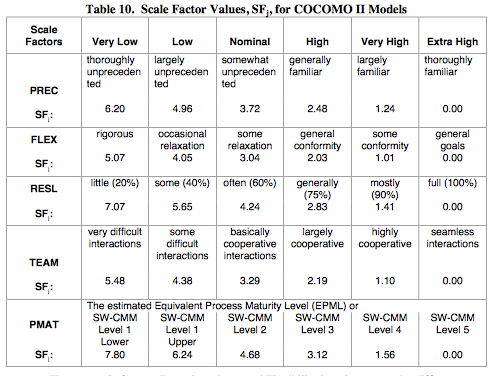
\includegraphics[trim={0.23cm 0.2cm 0.43cm 0.55cm},clip,width=\linewidth]{img/scaledriver.png}
    \caption{Scale Factor Values for COCOMO II Models}
    \label{tbl:scale}
\end{figure}

\pagebreak 
In this section we'll talk about COCOMO II Scale Drivers. They are a significant
source of exponential variation on project's effort. Each driver has a range of 
rating levels, from Very Low to Extra High, each with its own rate. 

\paragraph{PREC} Precedentedness. \\ 
This driver reflects the previous experience that the developers have in this 
field. Actually, this is our first experience, so we think the best value for
our team is \emph{LOW}.

\paragraph{FLEX} Development flexibility. \\
This driver will change due to our flexibility degree in the development.
Our schedule is quite strict, so we choose \emph{LOW} for this project.

\paragraph{RESL} Risk resolution. \\
% TODO!!
It reflects the extension of the risk analysis. We choose 'generally'
because reasons. % <- TODO

\paragraph{TEAM} Team cohesion. \\
This value is correlated to how well the development team know each other. 
In this case we are a very cooperative team, so \emph{VERY HIGH} value is
our choice.

\paragraph{PMAT} Process maturity. \\
% TODO!!
Here there is the weighted average of ``Yes'' answers to CMM Maturity Questionnaire.
Let's Try with High, Level 3

Here is a sum of archieved results.

\begin{tabular}{ p{5cm} | c | c }
    Scale Driver            & Factor             &  Value   \\ \hline
    Precedentedness         & \texttt{LOW}       &  4.96    \\
    Development Flexibility & \texttt{LOW}       &  4.05    \\
    Risk Resolution         & \texttt{HIGH}      &  2.83    \\
    Team Cohesion           & \texttt{VERY HIGH} &  1.10    \\
    Proces Maturity         & \texttt{HIGH}      &  3.12    \\ \hline
    Total                   &                    & 16.06  
\end{tabular}

\pagebreak
\subsection{Cost Drivers} % (fold)
These are the efforti multipliers used in COCOMO II model to adjust the
nominal effort. 
\label{sub:cost_drivers}

\cost{RELY}{Required Software Reliability}
{Slight inconvenience}{Easily recoverable losses}{Easily recoverable losses}
{High financial loss}{Risk to human life}{}
{0.82}{0.92}{1.00}{1.10}{1.26}{n/a} {
    This is the measure of software reliability. \emph{NORMAL} is our choice
    for this case because a downtime would not lead to high financial losses
    but will cause problems to passengers.
}
\cost{DATA}{Database Size}
{ }{D/P < 10}{$ 10 \leq D/P \le 100 $}{ $ 100 \leq D/P \le 1000 $} { $ D/P \ge 1000 $ } { }
{n/a}{0.90}{1.00}{1.14}{1.28}{n/a}
{This values tries to estimate effects that large databases could have in our application.
    We do not have a test database, so we use \emph{Nominal} as value.
}
\scost{CPLEX}{Product Complexity} { 0.73}{0.87}{1.00}{1.17}{1.34}{1.74} { 
    According to \emph{Table 20} 
    \footnote{ \url{http://sunset.usc.edu/research/COCOMOII/expert/cocomo/drivers.html} }
    our software could be marked as \emph{Nominal}.
}

\cost{RUSE}{Required Reusability}
{ } { None } { Across project } { Across program } { Across product line} 
{Across multiple product lines} { n/a}{0.95}{1.00}{1.07}{1.15}{1.24} {
    Reusability is useful. Some parts should be designed as reusable (e.g.
    Mobile communication drivers). Those parts could be used not only in this project. \\
    \emph{High} is our choice here.
}

\cost{DOCU}{Documentation match to life\-cycle needs}
{Many life\-cycle needs uncovered.}{Some life\-cycle needs uncovered.}
{Right\-sized to life\-cycle needs.}{Excessive for life\-cycle needs.}
{Very excessive for life\-cycle needs.}{ } 
{0.81}{0.91}{1.00}{1.11}{1.23}{ n/a } { 
    This is a cost driver for the level of required documentation. 
    In our case it is suitable as \emph{Nominal}.
}

\pagebreak

\scost{TIME}{Execution Time Constraint}{n/a}{n/a}{1.00}{1.11}{1.29}{1.63} {
    This is a measure of the execution time constraint. We don't have any
    constraint in this case, so we will set it as \emph{Very Low}.
}

\scost{STOR}{Main Storage Constraint}{n/a}{n/a}{1.00}{1.05}{1.17}{1.46} {
    This is a measure of the degree of main storage constraint. 
    We don't have any constraint, so we will set it as \emph{Very Low}.
}

\cost{PVOL}{Platform Volatility}{ }{Major: 12 months. Minor: 1 month.}
{ Major: 6 months. Minor: 2 weeks } { Major: 2 months. Minor: 1 weeks }
{ Major: 2 weeks. Minor: 2 days } { }
{n/a}{0.87}{1.00}{1.15}{1.30}{n/a} {
    Our estimation is that this is a stable system with low volatility.
    \emph{Low} is a good choice here.
}

\scost{ACAP}{Analyst Capability}{1.42}{1.19}{1.00}{0.85}{0.71}{n/a} {
    This driver should be set to \emph{High} since we dedicated a lot of
    effort in analysing the problem requirements.
}

\scost{PCAP}{Programmer Capability}{1.34}{1.15}{1.00}{0.88}{0.76}{n/a} {
    This driver should emphasize our programmers' capabilites as a team. 
    Our cooperation is quite good, so we set it as \emph{High}.
}

\cost{APEX}{Application Experience}
{ $ \leq $ 2 months } { 6 months } {1 year } {3 years} {6 years} { }
{1.22}{1.10}{1.00}{0.88}{0.81}{n/a} { 
    Our experience in this field is very low. So we set this value as \emph {Very Low}.
}

\cost{PLEX}{Platform Experience}
{ $ \leq $ 2 months } { 6 months } {1 year } {3 years} {6 years} { }
{1.19}{1.09}{1.00}{0.91}{0.85}{n/a} { 
    Our average knowledge about platforms as databases, UI, client/server architecture
    is around 1 year. We set this value as \emph{Nominal}.
}

\paragraph{Language and Tool Experience}
\paragraph{Personnell Continuity}
\paragraph{Usage of Software Tools}
\paragraph{Multisite Development}
\paragraph{Required development schedule}

% subsection cost_drivers (end)
% subsection scale_drivers (end)
\subsection{Effort Equation} % (fold)
\label{sub:effort_equation}
